\documentclass[a4paper]{article}
\usepackage[affil-it]{authblk}
\usepackage{graphicx}
\usepackage{amsfonts}
\usepackage{amsmath}
\usepackage[backend=bibtex,style=numeric]{biblatex}

\usepackage{geometry}
\geometry{margin=1.5cm, vmargin={0pt,1cm}}
\setlength{\topmargin}{-1cm}
\setlength{\paperheight}{29.7cm}
\setlength{\textheight}{25.3cm}

\addbibresource{citation.bib}

\begin{document}
% =================================================
\title{Numerical Analysis homework 1}

\author{Zirui Chen 22435036
  \thanks{Electronic address: \texttt{18107732576@163.com}}}
\affil{(24), Zhejiang University }


\date{Due time: \today}

\maketitle

%\begin{abstract}
 %   The abstract is not necessary for the theoretical homework, 
   % but for the programming project, 
    %you are encouraged to write one.      
%\end{abstract}





% ============================================
\section*{I}

$477 = (101001101)_{2}$


\section*{II}
$\frac{3}{5} = (1.0011001\cdots)_{2} \times 2^{-1}$


\section*{III}

Prove:

Because $x = 1.0\times \beta ^{e}$, $x_{R} = 1.0\cdots 01\times \beta ^{e}$,$x_{L} = 0.1\cdots 11\times \beta ^{e-1}$,
so, $x_{R} - x = \beta ^{e-(p-1)}$, $x_{L} - x = \beta ^{e-1-(p-1)}$, $x_{R} - x = \beta(x - x_{L})$.

\begin{flushright} % 右对齐
    $\square$ 
\end{flushright} 

\section*{IV}

\subsection*{IV-a}
IEEE754(2, 24, -126, 127)

$x_{R} = 1.001101\cdots 1010 \times 2^{-1}$

$x_{L} = 1.001101\cdots 1001 \times 2^{-2}$

$x_{R} - x = \frac{2}{5}\times 2^{-24}$, $x_{L} - x = \frac{3}{5}\times 2^{-24}$, 
so we should choose $x_{R}$ .$Rel(\frac{3}{5}) = \frac{\|x_{R} - x\|}{\|x\|} = \frac{2}{3}\times 2^{-24}$


\section*{V}

Using nearest rounding, error will not be more than half of the machine precision plus $\beta^{e}$. if we 
drop excess bits, the unit roundoff will be the same as the machine precision plus $\beta^{e}$..


\section*{VI}

According to the Theroem4.49, set $x = 1, y = cos\frac{1}{4}, \beta = 2$
then $1-\frac{y}{x} = (0.03108\cdots)_{2} = (0.000001)_{10}$
So, at least 6bits of precision are lost.


\section*{VII}

We can use Taylor expansion and double angle formular.


\section*{VIII}

$Cond_{f(x)} = \frac{\| x\| \cdot \| \bigtriangledown f\| }{\| f(x)\| }$

(a) $(x-1)^{a} \Rightarrow \| \frac{ax}{x-1} \| ,x\rightarrow 1$

(b) $lnx \Rightarrow \| \frac{1}{lnx} \| ,x\rightarrow 1$

(c) $e^{x} \Rightarrow \| x \| , x\rightarrow \infty $

(d) $arcCosx \Rightarrow \| \frac{x}{\sqrt{1-x^{2}}\cdot arcCosx } \| , x\rightarrow \pm 1 $



\section*{IX}

\subsection*{IX-a}

$cond_{f}(x) = \vert \frac{x\cdot e^{-x}}{1-e^{-x}}\vert = \vert \frac{x}{e^{x} - 1}\vert $
it is trival to show that $cond_{f}(x) \leq 1$ for $x \in (0,1)$.

\subsection*{IX-b}
According to Theroem4.40, we have, 
\begin{align}
f_{A}(x) &= fl(1 - fl(e_{-x})) \\ 
         &= (1 - e^{x}(1 + \delta_{1}))(1 + \delta_{2}) \\
         &= (1 - e^{-x})(1 + \delta_{2} - \delta_{1}\frac{1}{e^{x} - 1}) \\
\end{align}

where $\delta_{1}, \delta_{2} \leq \varepsilon_{u}$, set $\varphi(x) = \frac{1 - 2e^{-x}}{1 - e^{-x}}$

so, $cond_{A}(x) \leq \frac{\varphi(x)}{cond_{f}(x)} = \frac{e^{x}+2e_{-x}-3}{x(1-e^{-x})}$

\subsection*{IX-c}

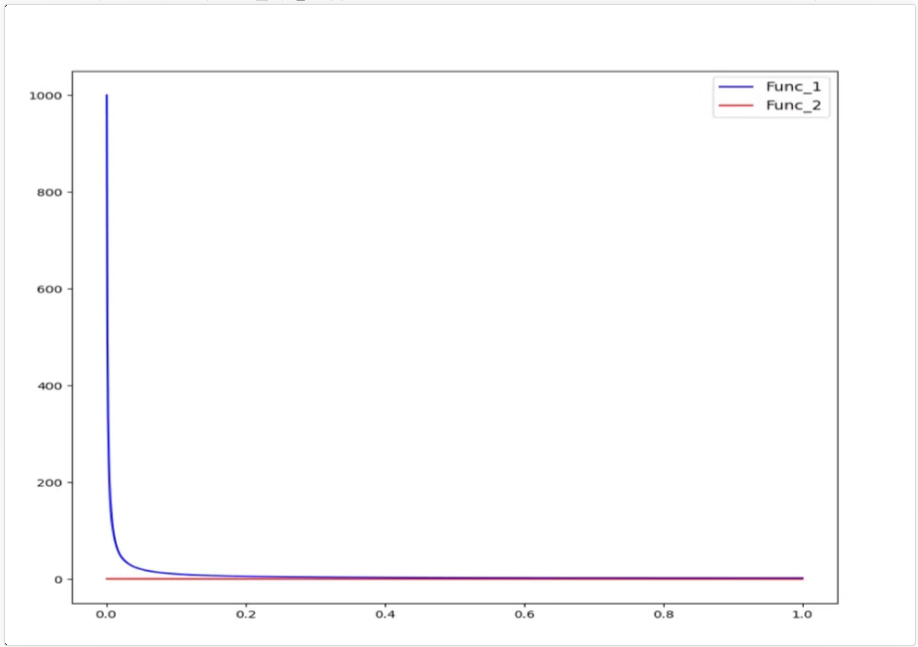
\includegraphics[width=0.8\textwidth]{pic.png}


\section*{X}

\section*{XI}
Prove:

$$cond_{f}(x) = \| [\frac{a_{0}}{r}\frac{\partial r}{\partial a_{0}}, \cdots, \frac{a_{n-1}}{r}\frac{\partial r}{\partial a_{n-1}}] \|_{1}$$

$\frac{\partial r}{\partial a_{k}} = r^{k} + \frac{\partial r}{\partial a_{k}}q^{'}(r) \Rightarrow \frac{\partial r}{\partial a_{k}} = -\frac{r_{k}}{q^{'}(r)}$

Because the  1-norm and the infinity norm are equivalent.consider the 1-norm, 
when $q(x) = \prod_{k=1}^{p}(x-k)$, we have, $cond_{q}(r) = \frac{r^{n-1}}{\prod ^{n}_{k=1,k\neq r}\mid r-k\mid }$
So when r = n. $cond_{p}(r) \rightarrow \infty$

\begin{flushright} % 右对齐
    $\square$ 
\end{flushright} 


\section*{XII}
Set $(2,2,-1,1), a=1.0\times 2^{0}, b = 1.1\times 2^{0}, \frac{a}{b} = \frac{10}{11}$
$$M = fl_{register}(\frac{1.0}{1.1}) = fl_{register}((0.1010\cdots)_{2}) = (0.101)_{2}$$
and $fl(1.01\times 2^{-1}) = 1.0\times 2^{-1}$, so $e_{rel} = \frac{9}{20} > \frac{1}{2}\varepsilon_{M} = \frac{1}{4}$


\section*{XIII}

Prove:

In IEEE754, \varepsilon _{u} = \frac{1}{2}\varepsilon _{M} = 2^{-24}

Because $128 = (10000000)_{2} = 1.0 \times 2^{7}$, and $129 = (10000001)_{2} = (1.0000001) \times 2^{7}$.

So, $\max_{x}E(x) = \geq \varepsilon _{M}\times 2^{7} = (1.0)_{2} \times 2^{-17} \geq 10^{-6}$

Thus ,we cant find root with error less than $10^{-6}$ in this range.

\section*{XIV}
Prove:

when $x_{i+1} - x_{i}$is much smaller than those of other adjacent pairs.
% Denote $x_{i+1} - x_{i} = \delta_{i}$.

% Consider spline $S_{i}(x), x\in [x_{i},x_{i+1}]$, we have$S_{i}(x) = f_{i} + a_{0}(x-x_{i}) + a_{1}(x - x_{i})^{2} + a_{2}(x - x_{i})^{3}$.
% express as matrix form, we have
% $$\begin{bmatrix}
%     \delta_{i} & \delta_{i}^{2} & \delta_{i}^{3} \\
%     0 & 2\delta_{i} & 3\delta_{i}^{2} \\
% \end{bmatrix}
% \begin{bmatrix}
%     a_{0} \\
%     a_{1} \\
%     a_{2} \\
% \end{bmatrix}
% = \begin{bmatrix}
%     f_{i+1} - f_{i} \\
%     f_{i+2} - f_{i+1} \\
% \end{bmatrix}$$
the coefficent matrix of the interpolating polynomial is ill-conditioned.

% ===============================================
\section*{ \center{\normalsize {Acknowledgement}} }
Give your acknowledgements here(if any).

\end{document}